\documentclass[a0paper,fontscale=0.3]{baposter}  % fontscale=0.285, dvipdfm

\usepackage{setspace}
\usepackage{multicol}
\usepackage{multirow}

%\usepackage{tikz}
%\usepackage{pgfbaselayers}
%\pgfdeclarelayer{background}
%\pgfdeclarelayer{foreground}
%\pgfsetlayers{background,main,foreground}

%%% Color Definitions %%%%%%%%%%%%%%%%%%%%%%%%%%%%%%%%%%%%%%%%%%%%%%%%%%%%%%%%%

%\definecolor{bordercol}{RGB}{40,40,40}
%\definecolor{bordercol}{RGB}{100,0,0}
\definecolor{bordercol}{RGB}{0,0,0}
%\definecolor{headercol1}{RGB}{186,215,230}
%\definecolor{headercol2}{RGB}{80,80,80}
%\definecolor{headercol1}{RGB}{153,0,0}
%\definecolor{headercol2}{RGB}{153,0,0}
\definecolor{headercolone}{RGB}{6,130,22}
\definecolor{headercoltwo}{RGB}{6,130,22}
%\definecolor{boxcolor}{RGB}{186,215,230}
%\definecolor{boxcolor}{RGB}{110,230,209}
%\definecolor{boxcolor}{RGB}{143,255,236}
%\definecolor{boxcolor}{RGB}{171,255,241}
\definecolor{boxcolor}{RGB}{176,232,223}
\definecolor{headerfontcol}{RGB}{255,255,255}
%\definecolor{boxcolor}{RGB}{186,215,230}
%\definecolor{boxcolor}{RGB}{226,200,200}
%\newcommand{\hilitetwo}[1]{{\addfontfeature{Color=FF000099}#1}}
\newcommand{\hilitetwo}[1]{{\addfontfeature{Color=99333399}#1}}
%\newcommand{\hiliteone}[1]{{\addfontfeature{Color=33993399}#1}}
\newcommand{\hiliteone}[1]{{\addfontfeature{Color=06821699}#1}}
\newcommand{\hilitegrey}[1]{{\addfontfeature{Color=77777799}#1}}

%%% Utility functions %%%%%%%%%%%%%%%%%%%%%%%%%%%%%%%%%%%%%%%%%%%%%%%%%%%%%%%%%%

%%% Save space in lists. Use this after the opening of the list %%%%%%%%%%%%%%%%
\newcommand{\compresslist}{
        \setlength{\itemsep}{1pt}
        \setlength{\parskip}{0pt}
        \setlength{\parsep}{0pt}
}

\usepackage{polyglossia}
\setdefaultlanguage[variant=australian]{english}

\usepackage{expex}

\usepackage{fontspec}
\defaultfontfeatures{PunctuationSpace=3,Scale=MatchLowercase,Mapping=tex-text}
\newfontfeature{IPA}{+mgrk}
%\setromanfont[IPA]{FreeSerif}
%\setromanfont[IPA,Scale=0.8]{CMU Serif}
\setromanfont[IPA]{Liberation Serif}
%\setromanfont[IPA]{Times New Roman}
%\setromanfont[IPA]{NimbusRomNo9L-Regu}
%\setromanfont{Times New Roman}
%\setmonofont[IPA]{Liberation Mono}
\setmonofont[IPA]{DejaVu Sans Mono}
%\renewcommand{\sfdefault}{phv}
%\renewcommand{\rmdefault}{ptm}
%\renewcommand{\ttdefault}{pcr}
\usepackage[small,bf]{caption}
%\newfontfamily\qipa[IPA]{NimbusRomNo9L-Regu}
\newfontfamily\qipa[IPA,Scale=MatchLowercase]{FreeSerif}
\newfontfamily\qgmk[IPA,Scale=0.8]{CMU Serif}

\newcommand{\tilda}{{\qipa ∼}}

\newcommand{\tags}[1]{\hiliteone{#1}}
\newcommand{\tag}[1]{\hilitegrey{<}\hiliteone{#1}\hilitegrey{>}}

%\newfontfamily\htwo[IPA,Scale=1.2]{FreeSans}}
%\newfontfamily\htwofont[IPA,Scale=1]{CMU Sans Serif}
%\newfontfamily\htwofont[IPA,Scale=1,Color=333344FF]{CMU Sans Serif}
\newfontfamily\htwofont[IPA,Scale=1,Color=111111FF]{CMU Sans Serif}
%\newfontfamily\titlefont[IPA,Scale=0.52]{CMU Serif}
\newfontfamily\titlefont[IPA,Scale=0.7]{CMU Serif}
%\newfontfamily\titlefont[IPA,Scale=0.55]{DejaVu Serif}

%\newcommand{\htwo}[1]{::: {\htwofont #1} :::}%\hrule} %\hline\\}
%\newcommand{\htwo}[1]{{\htwofont \textbf{:::#1:::}}}%\hrule} %\hline\\}
\newcommand{\htwo}[1]{{\htwofont \textbf{\dotfill{}#1\dotfill{}}}}


\usepackage{graphicx}  % [dvipdfm]

%\definecolor{MyGray}{rgb}{0.96,0.97,0.98}
%\newenvironment{codebox}{%
%   \begin{lrbox}{\@tempboxa}\begin{minipage}{\columnwidth}}{\end{minipage}\end{lrbox}%
%   \colorbox{MyGray}{\usebox{\@tempboxa}}
%}
%\newcommand{\codeex}[1]{\begin{codebox}#1\end{codebox}}

%\definecolor{grey}{rgb}{0.96,0.97,0.98}
\definecolor{grey}{rgb}{0.91,0.91,0.91}
\newcommand{\codeex}[1]{
   \fbox{\colorbox{grey}{
         \begin{minipage}[t]{0.91\textwidth}
            #1
         \end{minipage}
      }
   }
}

\newcommand{\blank}[1]{\underline{\hspace{#1}}}
% FIXME: Breaks baposter
%\usepackage[novoc,fdf2alif]{arabxetex}
%\newfontfamily\uighurfont[Script=Arabic,Scale=1.5]{Lateef}
%\newfontfamily\arabicfont[Script=Arabic,Scale=1.5]{Lateef}

\usepackage{natbib}

%\makeatletter
%\renewenvironment{thebibliography}[1][]{\htwo{\bibname}}
%     {\section*{\bibname}% <-- this line was changed from \chapter* to \section*
%	  \htwo{\bibname}
%      \@mkboth{\MakeUppercase\bibname}{\MakeUppercase\bibname}%
%      \list{\@biblabel{\@arabic\c@enumiv}}%
%           {\settowidth\labelwidth{\@biblabel{#1}}%
%            \leftmargin\labelwidth
%            \advance\leftmargin\labelsep
%            \@openbib@code
%            \usecounter{enumiv}%
%            \let\p@enumiv\@empty
%            \renewcommand\theenumiv{\@arabic\c@enumiv}}%
%      \sloppy
%      \clubpenalty4000
%      \@clubpenalty \clubpenalty
%      \widowpenalty4000%
%      \sfcode`\.\@m}
%     {\def\@noitemerr
%       {\@latex@warning{Empty `thebibliography' environment}}%
%      \endlist}%}
%}
%\makeatother
%\usepackage[in]{fullpage}
\usepackage[colorlinks=true,citecolor=black,linkcolor=black,urlcolor=black]{hyperref}

\usepackage{subfigure}
\usepackage{booktabs}

%%\bibpunct{(}{)}{;}{A}{,}{,}
%\bibdata{paper}

\newcommand{\citemultileft}[1]{(\citeauthor{#1}, \citeyear{#1}}
\newcommand{\citemultimid}[1]{\citeauthor{#1}, \citeyear{#1}}
\newcommand{\citemultiright}[1]{\citeauthor{#1}, \citeyear{#1})}
\newcommand{\citetwoyears}[2]{\citeauthor{#1} (\citeyear{#1} and \citeyear{#2})}

% for glosses
\newcommand{\eng}[1]{`{\em #1}'}
%dammit, sc doesn't seem to be working
\newcommand{\gmk}[1]{{\qgmk \textsc{#1}}}


\usepackage{enumitem}
\setlist{nolistsep,leftmargin=*}
\newenvironment{itemise}[1]{
        \begin{itemize}\setlength{\leftmargin}{-4em}\setlength{\itemsep}{-0.2em}
        \vspace{-0.5em}
        #1
}{
        \end{itemize}
        \vspace{-2pt}
}

%\newcommand{\h2}[1]{{\big



\begin{document}
	% To get it to be A0 consistently on all machines..
	%\special{papersize=1189mm,841mm}
	\special{papersize=841mm,1189mm}
	\setlength{\pdfpageheight}{\paperheight}
	\setlength{\pdfpagewidth}{\paperwidth}

%%% Setting Background Image %%%%%%%%%%%%%%%%%%%%%%%%%%%%%%%%%%%%%%%%%%%%%%%%%%
%\background{
%	\includegraphics[width=0.99\textwidth]{flagkg2}
%}
	\background{{
%		\begin{tikzpicture}[remember picture,overlay]%
%			\draw (current page.north west)+(-4em,2em) node[anchor=north west] {\includegraphics[width=1.1\textwidth,height=1.1\textheight]{flagkg2}};
%		\end{tikzpicture}%
%%		\includegraphics[width=0.99\textwidth]{flagkg2}
%%			\draw (current page.north west)+(-2em,2em) node[anchor=north west] {\includegraphics[width=0.9\textwidth]{flagkg2}};
	}}



	\begin{poster}{
			grid=false,
			%eyecatcher=false,
			borderColor=bordercol,
			headerColorOne=headercolone,
			headerColorTwo=headercoltwo,
			headerFontColor=white,
			% Only simple background color used, no shading, so boxColorTwo isn't necessary
			boxColorOne=boxcolor,
			headershape=roundedright,
  headerborder=open,
  headerheight=0.08\textheight,
  %headershape=roundedright,
  %headershade=plain,
  %headerfont=\Large\textsf, %Sans Serif
			%headerfont=\Large\sf\bf,
			textborder=rectangle,
			%background=plain,
			%background=user,
			background=none,
			headerborder=open,
			boxshade=plain,
			textborder=roundedleft,
		}{
			%\hspace{-2em}\includegraphics[height=6.5em,bb=0 0 242 203]{apertium}
			%\hspace{-2em}\includegraphics[height=6.5em,bb=0 0 612 792]{apertium2}
			%\hspace{-2em}\includegraphics[height=6.5em,bb=0 0 203 242]{apertium3}
			%\hspace{-2em}\includegraphics[height=6.5em,bb=0 0 242 203]{apertium3a}
			%\hspace{-2em}\includegraphics[height=6.5em,bb=0 0 242 203]{apertium4}
			\hspace{-2em}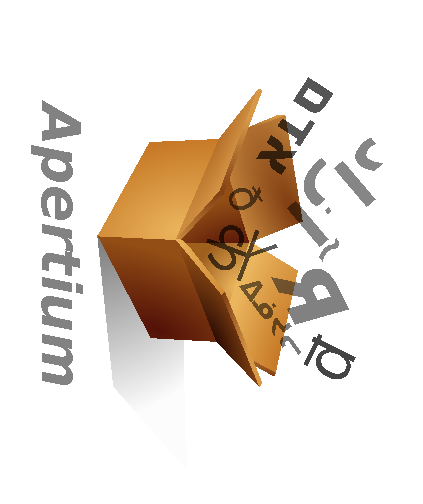
\includegraphics[angle=90,height=7.5em]{apertium5a}
			%Eye Catcher, empty if option eyecatcher=false - unused
		}{
			{\vspace{0pt}\hspace{-2.2ex}
			{\titlefont \textsc{Finite-state morphological transducers\\for three Kypchak languages}}}
		}{
			%Jonathan North Washington {\small (Indiana University, \texttt{jonwashi@indiana.edu})}, Mirlan Ipasov {\small (International Ataturk Alatoo University, \texttt{mipasov@gmail.com})}, Francis M.\ Tyers {\small (Universitat d'Alacant, \texttt{ftyers@dlsi.ua.es})}

			\vspace{-0.5em}
			\begin{center}
			{\begin{minipage}[t]{11.2em}
				\begin{spacing}{0.4}
					{Jonathan North Washington}\\
					{\footnotesize Indiana University\\\texttt{jonwashi@indiana.edu}}
				\end{spacing}
			\end{minipage}
			\begin{minipage}[t]{10.5em}
				\begin{spacing}{0.4}
					{Ilnar Salimzyanov}\\
					{\footnotesize Казан (Идел буе) федераль университеты \\\texttt{ilnar.salimzyan@gmail.com}}
				\end{spacing}
			\end{minipage}
			\begin{minipage}[t]{8.2em}
				\begin{spacing}{0.4}
					{Francis M.\ Tyers}\\
					{\footnotesize UiT Norgga Árktalaš Universitehta \\\texttt{francis.tyers@uit.no}}
				\end{spacing}
			\end{minipage}}
			\begin{minipage}[t]{5.5em}
				\begin{spacing}{0.4}
					{\footnotesize Special thanks to}\\
					{\small Aida Sundetova}\\
					{\footnotesize \texttt{sun27aida@gmail.com}}
				\end{spacing}
			\end{minipage}
			\end{center}

			%\begin{minipage}[c]{12em}
			%	\centering
			%	\begin{spacing}{0.4}
			%		Jonathan Washington\\
			%		Indiana University\\
			%		\texttt{jonwashi@indiana.edu}
			%	\end{spacing}
			%\end{minipage}
			%\begin{minipage}[c]{18em}
			%	\centering
			%	\begin{spacing}{0.4}
			%		Mirlan Ipasov\\
			%		International Ataturk Alatoo University\\
			%		\texttt{mipasov@gmail.com}
			%	\end{spacing}
			%\end{minipage}
			%\begin{minipage}[c]{10em}
			%	\centering
			%	\begin{spacing}{0.4}
			%		Francis M.\ Tyers\\
			%		Universitat d'Alacant\\
			%		\texttt{ftyers@dlsi.ua.es}
			%	\end{spacing}
			%\end{minipage}

			%Jonathan Washington, Mirlan Ipasov, Francis M.\ Tyers\\
			%Indiana University, Universitat d'Alacant, International Ataturk Alatoo University\\
			%\texttt{jonwashi@indiana.edu}, \texttt{mipasov@gmail.com}, \texttt{ftyers@dlsi.ua.es}
		}{
			%University Logo(s)
			%{\begin{minipage}{19em}
				%\hfill
				%\includegraphics[height=6.5em]{apertium}
				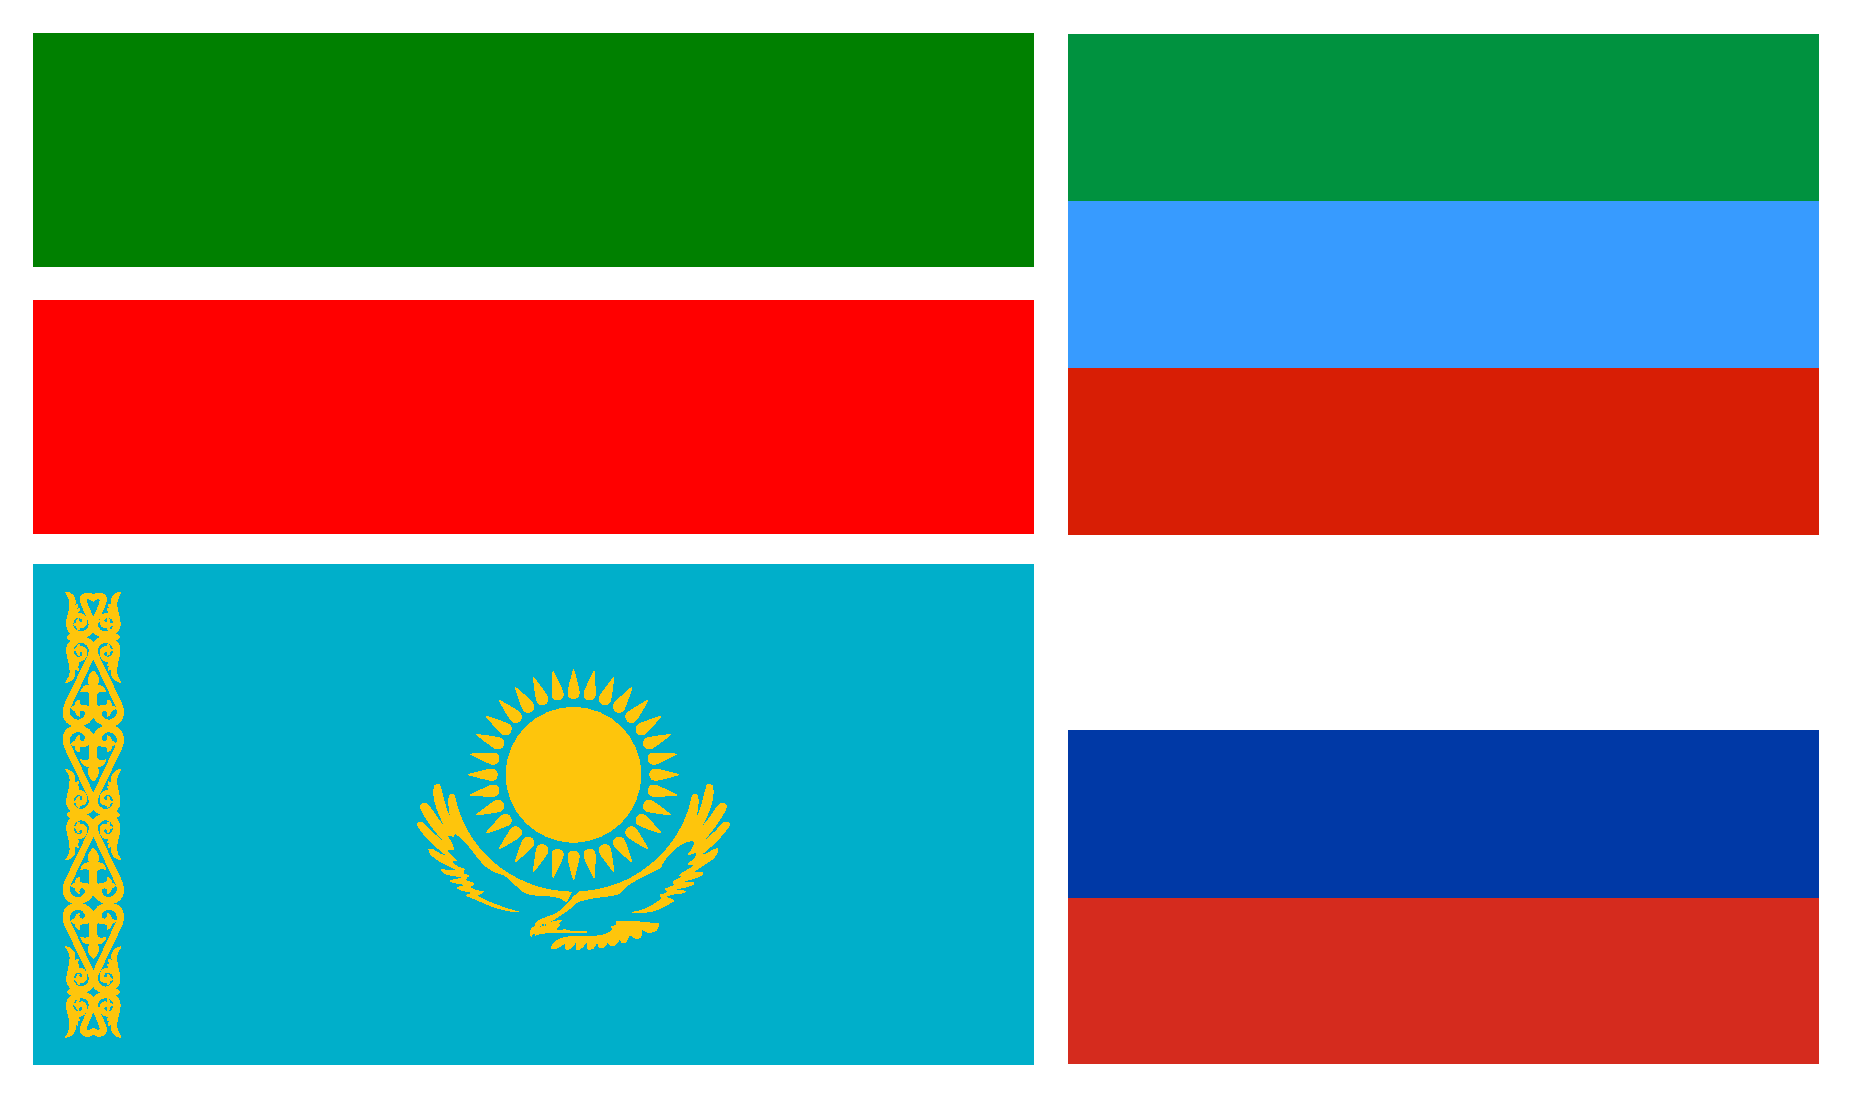
\includegraphics[height=6.5em]{flags/flags}
			%\end{minipage}}
		}

%		\headerbox{Overview}{name=overview,column=0,row=1}{
%			\begin{spacing}{0.8}
%This paper describes the development of a free/open-source finite-state morphological transducer for Kyrgyz. The transducer 
%has been developed for morphological generation for use within a prototype Turkish$\rightarrow$Kyrgyz machine translation system, but has also been extensively tested for analysis. The finite-state toolkit used for the work was the Helsinki Finite-State 
%Toolkit (HFST). The paper describes some issues in Kyrgyz morphology, the development of the tool, some linguistic issues encountered and how they were dealt with, and 
%which issues are left to resolve. An evaluation is presented which shows that the transducer has medium-level coverage, between 82\% and 87\% on two freely available corpora of Kyrgyz, and high precision and recall over a manually verified test set.
%			\end{spacing}\vspace{-0.25ex}
%		}

	\headerbox{Kypchak languages}{name=kypchaklgs,column=0,row=0}{
		\vspace{0.5ex}
		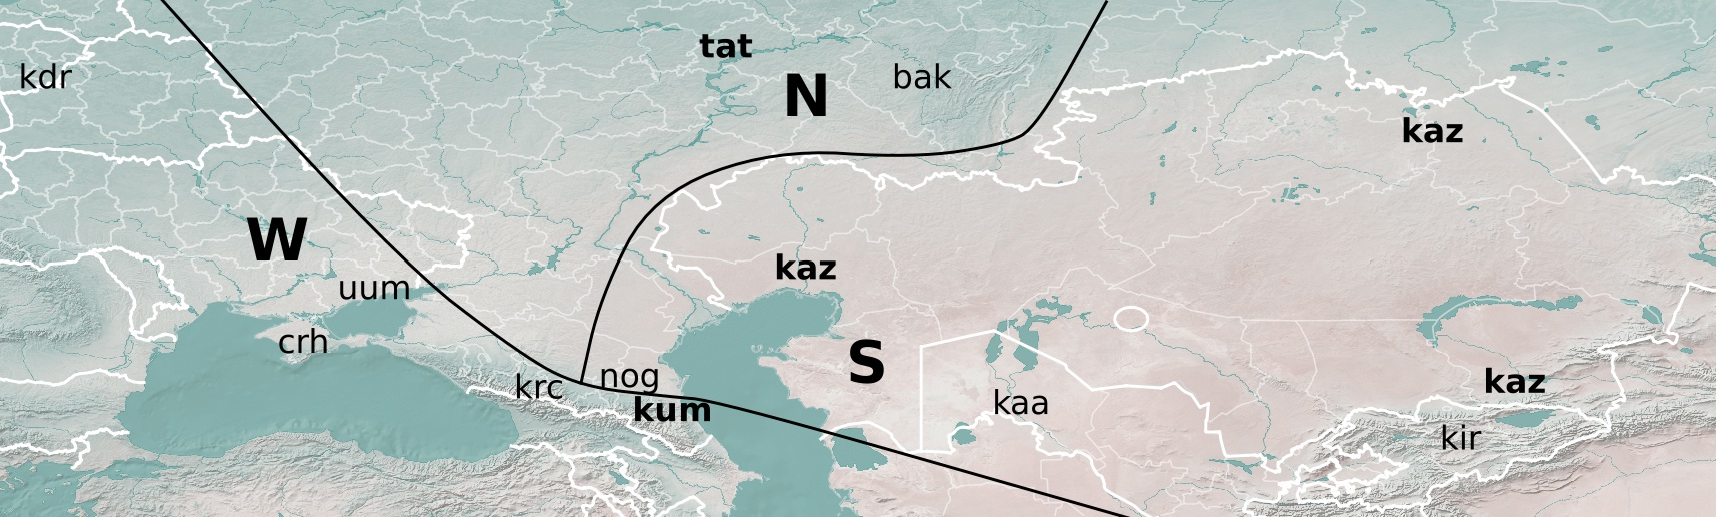
\includegraphics[width=\textwidth]{map}
		\vspace{-1.1em}  % -1.25em
		\begin{itemize}
			\item Turkic languages (SOV, agglutinative, vowel harmony)
		\end{itemize}

	\scalebox{0.85}{
		\begin{tabular}{llll}
			\toprule
				 & \textbf{Kazakh} & \textbf{Tatar} & \textbf{Kumyk} \\
				 & /{\qipa qɑzɑq}/ & /{\qipa tɒtɑɾ}/ & /{\qipa qumuq}/ \\
				classif'tion & S Kypchak & N Kypchak & W Kypchak \\
			\midrule
				\multicolumn{4}{l}{population of speakers} \\
			\midrule
				number & 8M-12M & 5.4M & 430K \\
				primary & Kazakhstan & Tatarstan & Dagestan \\
				secondary & China, Mongolia & Bashqortostan & --- \\
			\midrule
				\multicolumn{4}{l}{external influences} \\
			\midrule
				Mongolic & moderate & light & light \\
				Oghuz & — & light & moderate \\
				Persian & heavy & heavy & heavy \\
				Russian & heavy & heavy & heavy \\
			\bottomrule
		\end{tabular}
	}
%			\begin{itemize}
%				\item Similar historically to Southern Altay
%				\item Similar by convergence to Kazakh, Uzbek
%			\end{itemize}
%			\item Spoken in
%			\begin{itemize}
%				\item Kyrgyzstan, as co-official language\\
%				\textit{high levels of bilingualism with Russian}
%				\item China, Tajikistan, Uzbekistan
%			\end{itemize}
%			\item Over 3 million native speakers\\(estimate based on data from Ethnologue) %\citep{lewis2009}
%			\item Our transducer based on written Kyrgyz of the former Soviet Union (literary and colloquial standards)
%		\end{itemize}
	}
	
	\headerbox{Morphological transducers}{name=morphtrans,below=kypchaklgs}{
		\htwo{Morphological transducers}
		\begin{itemize}
			\item Take a surface form, and produce valid lexical form(s)
			\item Take a lexical form, and produce valid surface form(s)
		\end{itemize}
		\scalebox{0.96}{
			`алдым' \hilitetwo{↔} \texttt{ал{\small <v><tv><ifi><p1><sg>}}, \texttt{алд{\small <n><px1sg><nom>}}
		}

		\htwo{Transducers for Turkic languages}
		\begin{itemize}
			\item Turkish (\hiliteone{Çöltekin, 2010 \& 2014}; \hilitetwo{Öflazer, 1994})
			\item Crimean Tatar (\hilitetwo{Altıntaş, 2001})
			\item Turkmen (\hilitetwo{Tantuğ et al., 2006})
			\item Kyrgyz (\hiliteone{Washington et al., 2012})%\\
			%\vspace{1pt}\hfill{} \hiliteone{GPL (=free and open)}!
			\item Kazakh, Tatar, Kumyk: all \hiliteone{GPL (=free and open)}!
		\end{itemize}

		\htwo{Framework: HFST}
		\begin{itemize}
			\item Reimplements Xerox FST formalisms ({\tt lexc} \& {\tt twol})
			\item Also provides a wrapper around popular free/open-source FST toolkits: SFST, OpenFST, and Foma
		\end{itemize}

		\htwo{Development effort}
		\begin{itemize}
			\item Kumyk transducer based on Kazakh, Tatar transducers
			\item \tilda{}1 week to reach 80\% coverage, +1 week to reach 90\%
		\end{itemize}
		\vspace*{-2em}
		\hspace*{-2em}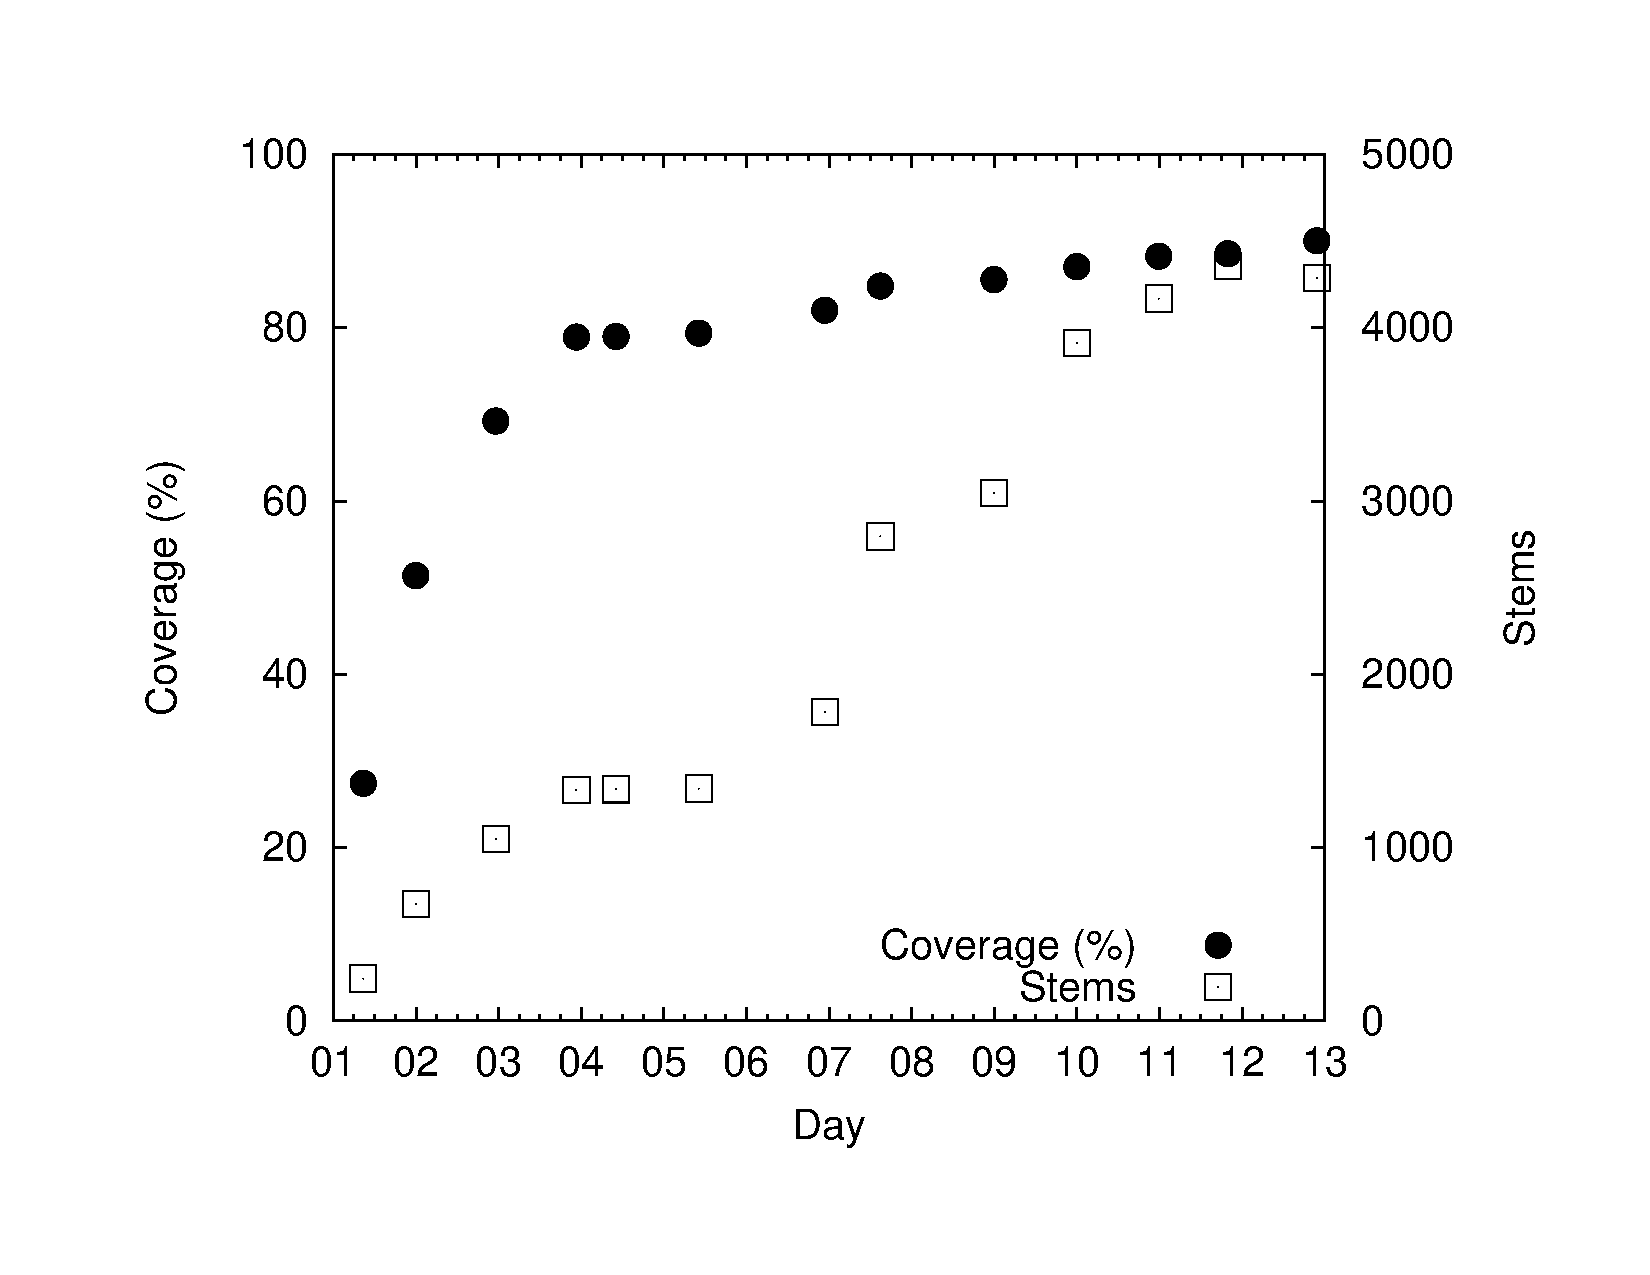
\includegraphics[width=0.9\textwidth,angle=270]{../graphs/kumyk-yoldash-cov}
		\vspace*{-2em}
	}

%		\headerbox{Available Turkic Transducers}{name=turkictrans,below=morphtrans}{
%* Other Turkic morphological transducers\\
%		}
%		\headerbox{Framework: HFST / Apertium}{name=framework,below=turkictrans}{
%* HFST/Apertium
%		}

		\headerbox{Categorisation}{name=lexc,below=morphtrans}{
		%\headerbox{Morphophonology}{name=morphophon,below=morphtrans}{
			\begin{itemize}
				\item Other Turkic transducers:\ \texttt{0}-derivation (\hilitetwo{overgenerates})
				\item Our approach:\ categorization (e.g., adjectives, below)
			\end{itemize}

		\scalebox{0.63}{
			\begin{tabular}{lllll}
				\toprule
				\textbf{Type} & \textbf{Gloss} & {\small \texttt{\tag{adj}(\tag{comp})}} & {\small \texttt{\tag{adj}\tag{subst}(\tag{comp})}} & {\small \texttt{\tag{adj}\tag{advl}(\tag{comp})}} \\
				\midrule
				A1 & \emph{`good'} & {\qipa яхшы (яхшырак)} & {\qipa яхшы (яхшырак)} & {\qipa яхшы (яхшырак)} \\
				A2 & \emph{`old'} & {\qipa иске (искерәк)} & {\qipa иске (искерәк)} & {\qipa — (—)} \\
				A3 & \emph{`dead'} & {\qipa үле (—)} & {\qipa үле (—)} & {\qipa — (—)} \\
				A4 & \emph{`basic'} & {\qipa төп (—)} & {\qipa — (—)} & {\qipa — (—)} \\
				\bottomrule
			\end{tabular}
		}
	}

%			\htwo{Morphological \& orthographical words}
%
%			\begin{itemize}
%				\item{} {\qipa өнүктүрөбүзбү ?} \eng{will we develop [it]?}\\
%				\texttt{ өнүк{\small <v><tv><caus><aor><p1><pl>+}бы{\small <qst>}}
%				\item{} {\qipa келатсаң} \eng{if you come}\\
%				\texttt{кел{\tt {\small <v><iv><prt\_impf>}}+жат{\small <vaux><gna\_cnd><p2><sg>}}
%			\end{itemize}
%
%
%			\codeex{
%			{\small
%			\texttt{LEXICON N-INFL-3PX-COMPOUND\\
%			\vspace{-0.5ex}\%<n\%>:\%>\%\{S\%\}\%\{I\%\}\%\{n\%\} GEN-POS ;}\\
%			
%			\texttt{LEXICON Nouns\\
%			\vspace{-0.5ex}аба\%\ ырайы:аба\%\ ырай\ N-INFL-3PX-COMPOUND ;\\\vspace{-0.5ex}\hspace{0.1pt}\hfill{}!\ "weather"\\
%			\vspace{-0.5ex}чакыруу\%\ кагазы:чакыруу\%\ кагаз\ N-INFL-3PX-\\\vspace{-0.5ex}\hspace{0.1pt}\hfill{}COMPOUND ;\ !\ "invitation"}}
%			}
%				
%		}

					\renewcommand{\arraystretch}{0.65}



		\headerbox{Example output}{name=exout,span=2,column=1,row=0}{

		\htwo{Gloss}

		\pex[aboveexskip=0pt,belowexskip=3pt,aboveglftskip=0pt]\label{ex:sent}
			\begingl
				\gla[everygla={\qipa }] Құдай Өзінің жаратқандарының бәріне қарап, {} өте жақсы екенін көрді. //
				\glb[everyglb={\qipa }] Аллаһ Үзе яраткан нәрсәләргә карап, аларның бик яхшы икәнен күрде. //
				\glb[everyglb={\qipa }] Аллагь Оьзю яратгъан затлагъа къарап, олар бек яхшы экенин гёрген. //
				\glb God own-his created [everything/thing-s]-to looked.at, they/their very good being saw. // 
				\glft \eng{God looked at everything he had created and saw that it was very good.} //
			\endgl
		\xe


		\htwo{Output}
\scalebox{0.81}{
\begin{tabular}{lll}
\toprule
 \textbf{Kazakh} (\textbf{kaz}) & \textbf{Tatar} (\textbf{tat}) & \textbf{Kumyk} (\textbf{kum}) \\
\midrule
\texttt{Құдай Өзінің жаратқандарының} & \texttt{Аллаһ Үзе яраткан нәрсәләргә карап,} & \texttt{Аллагь Оьзю яратгъан затлагъа} \\
\texttt{бәріне қарап, өте жақсы екенін көрді.} & \texttt{аларның бик яхшы икәнен күрде.} & \texttt{къарап, олар бек яхшы экенин гёрген.} \\
\midrule
 \texttt{Құдай\tag{n}\tag{nom}} & \texttt{Аллаһ\tag{n}\tag{nom}} & \texttt{Аллагь\tag{n}\tag{nom}} \\
 \texttt{Өз\tag{prn}\tag{ref}\tag{px3sp}\tag{gen}} & \texttt{Үз\tag{prn}\tag{ref}\tag{px3sp}\tag{nom}} & \texttt{Оьз\tag{prn}\tag{ref}\tag{px3sp}\tag{nom}} \\
 \texttt{жарат\tag{v}\tag{tv}\tag{ger\_past}\tag{pl}\tag{px3sp}\tag{gen}} & \texttt{ярат\tag{v}\tag{tv}\tag{gpr\_past}} & \texttt{ярат\tag{v}\tag{tv}\tag{gpr\_past}} \\
 \texttt{бәрі\tag{prn}\tag{qnt}\tag{px3sp}\tag{dat}} & \texttt{нәрсә\tag{n}\tag{pl}\tag{dat}} & \texttt{зат\tag{n}\tag{pl}\tag{dat}} \\
 \texttt{қара\tag{v}\tag{tv}\tag{gna\_perf}} & \texttt{кара\tag{v}\tag{tv}\tag{gna\_perf}} & \texttt{къара\tag{v}\tag{tv}\tag{gna\_perf}} \\ 
\texttt{,\tag{cm}} & \texttt{,\tag{cm}} & \texttt{,\tag{cm}} \\
 ---      & \texttt{алар\tag{prn}\tag{pers}\tag{p3}\tag{pl}\tag{gen}} & \texttt{олар\tag{prn}\tag{pers}\tag{p3}\tag{pl}\tag{nom}} \\
 \texttt{өте\tag{adv}} & \texttt{бик\tag{adv}} & \texttt{бек\tag{adv}} \\
 \texttt{жақсы\tag{adj}} & \texttt{яхшы\tag{adj}} & \texttt{яхшы\tag{adj}} \\
 \texttt{е\tag{cop}\tag{ger\_past}\tag{px3sp}\tag{acc}} & \texttt{и\tag{cop}\tag{ger\_past}\tag{px3sp}\tag{acc}} & \texttt{э\tag{cop}\tag{ger\_past}\tag{px3sp}\tag{acc}} \\
 \texttt{көр\tag{v}\tag{tv}\tag{ifi}\tag{p3}\tag{sg}} & \texttt{күр\tag{v}\tag{tv}\tag{past}\tag{p3}\tag{sg}} & \texttt{гёр\tag{v}\tag{tv}\tag{past}\tag{p3}\tag{sg}} \\  
 \texttt{.\tag{sent}} & \texttt{.\tag{sent}} & \texttt{.\tag{sent}} \\
\bottomrule
\end{tabular}
}

		\htwo{Tagset}

\vspace{-1.5em}
\setlength{\columnsep}{-1em}
\setlength{\topsep}{-\parskip}
%\spacing{0.8}
\begin{multicols}{4}
\begin{tabbing}
  \texttt{{\small \tag{n}}}\hspace{1.5em} \=  Noun\\[-0.5ex]
%  \texttt{{\small <np>}} \> Proper noun\\[-0.5ex]
  \texttt{{\small \tag{v}}} \>  Verb\\[-0.5ex]
  \texttt{{\small \tag{prn}}} \> Pronoun \\[-0.5ex]
  \texttt{{\small \tag{det}}} \>  Determiner\\[-0.5ex]
%  \texttt{{\small <cnjcoo>}} \> Coord. conjunct.\\[-0.5ex]
%  \texttt{{\small <cnjadv>}} \> Adv. conjunct.\\[-0.5ex]
  \texttt{{\small \tag{adj}}} \> Adjective\\[-0.5ex]
  \texttt{{\small \tag{adv}}} \> Adverb\\[-0.5ex]
%  \texttt{{\small <vaux>}} \> Auxiliary verb\\[-0.5ex]
%  \texttt{{\small <cop>}} \> Copula\\[-0.5ex]
  \texttt{{\small \tag{iv}}} \> Intransitive\\[-0.5ex]
  \texttt{{\small \tag{tv}}} \> Transitive\\[-0.5ex]
%  \texttt{{\small <p2>}} \> Second person\\[-0.5ex]
  \texttt{{\small \tag{p3}}} \> Third person\\[-0.5ex]
%  \texttt{{\small <ant>}} \> Anthroponym\\[-0.5ex]
%  \texttt{{\small <dem>}} \> Demonstrative\\[-0.5ex]
%  \texttt{{\small <m>}} \> Masculine\\[-0.5ex]
%  \texttt{{\small <sg>}} \> Singular\\[-0.5ex]
  \texttt{{\small \tag{pl}}} \> Plural\\[-0.5ex]
  \texttt{{\small \tag{nom}}} \> `Nominative'\\[-0.5ex]
  \texttt{{\small \tag{gen}}} \> Genitive\\[-0.5ex]
  \texttt{{\small \tag{acc}}} \> Accusative\\[-0.5ex]
  \texttt{{\small \tag{dat}}} \> Dative\\[-0.5ex]
  \texttt{{\small \tag{qnt}}} \> Quantifier \\[-0.5ex]
%  \texttt{{\small \tag{itg}}} \> Interrogative \\[-0.5ex]
  \texttt{{\small \tag{ref}}} \> Reflexive \\[-0.5ex]
  \texttt{{\small \tag{pers}}} \> Personal \\[-0.5ex]
%  \texttt{{\small <loc>}} \> Locative\\[-0.5ex]
%  \texttt{{\small <px3sg>}} \> 3rd person poss. (Singular)\\[-0.5ex]
  \texttt{{\small \tag{cm}}} \> Comma\\[-0.5ex]
  \texttt{{\small \tag{sent}}} \> Sentence\\[-0.5ex]
%  \texttt{{\small <px3pl>}} \> 3rd person poss. (Plural)\\[-0.5ex]
%  \texttt{{\small <neg>}} \> Negative\\[-0.5ex]
%  \texttt{{\small <aor>}} \> Aorist\\[-0.5ex]
  \texttt{{\small \tag{past}}} \> Past (General) \\[-0.5ex]
  \texttt{{\small \tag{ifi}}} \> Past \\[-0.5ex]
  	\> \hspace{0.5em}(Eyewitness/Recent) \\[-0.5ex]
  \\[-0.5ex]
  \\[-0.5ex]
  \texttt{{\small \tag{px3sp}}} \hspace{1.1em} \= 3rd person poss.\\[-0.5ex]
  	\> \hspace{0.5em}(Singular/Plural)\\[-0.5ex]
%  \texttt{{\small <imp>}} \> Imperative\\[-0.5ex]
  \texttt{{\small \tag{gna\_perf}}} \> Verbal adverb \\[-0.5ex]
  	\> \hspace{0.5em}(Perfect)\\[-0.5ex]
  \texttt{{\small \tag{gpr\_past}}} \> Verbal adjective \\[-0.5ex]
  	\> \hspace{0.5em}(Past)\\[-0.5ex]
  \texttt{{\small \tag{ger\_past}}} \> Verbal noun (Past)
%  \texttt{{\small <prc\_impf>}} \> Participle (Imperfect)\\[-0.5ex]
%  \texttt{{\small <prc\_irre>}} \> Participle (Irrealis)\\[-0.5ex]
%  \texttt{{\small <prc\_real>}} \> Participle (Realis)\\[-0.5ex]
 
\end{tabbing}
\end{multicols}

		}

		\headerbox{Evaluation}{name=coverage,span=1,column=2,below=exout}{

			\htwo{Number of stems}
			%\vspace{-1.5em}
			\vspace{-0.5em}
			\begin{center}
			\begin{tabular}{lrrr}
				\toprule
				\multirow{2}{*}{\textbf{Part of speech}} & \multicolumn{3}{c}{\textbf{Number of stems}} \\ \cmidrule{2-4}
				& \textbf{Kazakh} & \textbf{Tatar} & \textbf{Kumyk} \\
				\midrule
				Noun & 2640 & 2795 & 2568 \\
				Verb & 1470 & 1143 & 386 \\
				Adjective & 754 & 816 & 219 \\
				Proper noun & 5701 & 5361 & 1443 \\
				Adverb & 171 & 177 & 63 \\
				Numeral & 63 & 63 & 44 \\
				Conjunction & 46 & 45 & 13 \\
				Postposition & 50 & 43 & 12 \\
				Pronoun & 32 & 28 & 17 \\
				Determiner & 39 & 34 & 9 \\
				\midrule
				Total: & \hiliteone{11224} & \hiliteone{10737} & \hiliteone{4845} \\
				\bottomrule
			\end{tabular}
			\end{center}
			%\vspace{2em}
			\vspace{-0.5em}


			\htwo{Test corpora}

%		\scalebox{0.8}{
%			\begin{tabular}{lll}
%				\toprule
%				\textbf{type} & \textbf{lang} & \textbf{contents} \\ % & \textbf{origin} \\
%				\midrule
%				Encyclopædic & kaz & Wikipedia \\ % wpdump & 20131006 \\
%					& tat & Wikipedia \\ % wpdump & 20130225 \\
%					& kum & — \\ % — & — \\
%				\midrule
%				News & kaz & RFE/RL (azattyq.org) \\ % RFE/RL & azattyq.org 2010 \\
%					& tat & tat.tatar-inform.ru \\ % Татар-информ & tat.tatar-inform.ru 2005-2011 \\
%					& kum & Ёлдаш (yoldash.etnosmi.ru) \\ % Ёлдаш & yoldash.etnosmi.ru \\
%				\midrule
%				Religion & kaz & Quran + Bible \\ % quran + bible & kkitap.net, kuran.kz \\
%					& tat & Quran + New Testament \\ % quran + nt & ibt.org.ru, tanzil.net \\
%					& kum & Genesis + New Testament \\ % genesis + nt & ibt.org.ru \\
%				\bottomrule
%			\end{tabular}
%		}
		\scalebox{0.73}{
			\begin{tabular}{llll}
				\toprule
					& \textbf{Wikipedia} & \textbf{News} & \textbf{Religion} \\
				\midrule
					\textbf{Kazakh} & Wikipedia & azattyk.org & Quran + Bible \\
					\textbf{Tatar} & Wikipedia & tat.tatar-inform.ru & Quran + New Testament \\
					\textbf{Kumyk} & --- & yoldash.etnosmi.ru & Genesis + New Testament \\
				\bottomrule
			\end{tabular}

%			\begin{tabular}{llll}
%				\toprule
%					& \textbf{Kazakh} & \textbf{Tatar} & \textbf{Kumyk} \\
%				\midrule
%					Wikipedia & Wikipedia & Wikipedia & --- \\
%					News & azattyq.org & tat.tatar-inform.ru & yoldash.etnosmi.ru \\
%					Religion & Quran + Bible & Quran + New Testament & Genesis + New Testament \\
%				\bottomrule
%			\end{tabular}
		}

%			\begin{itemize}
%				\item split into 10 equal parts; coverage calculated over each separately; standard deviation of mean calculated
%			\end{itemize}
			%both split into 10 equal parts; coverage calculated over each separately; standard deviation of the mean was calculated\\
			\htwo{Evaluation measures}
			\begin{itemize}
				\item \textbf{Naïve coverage} - percentage of surface forms in a given corpus receiving ≥ 1 analysis%\\(surface forms may have missing analyses)
				\item \textbf{Mean ambiguity} - average number of analyses for each surface form found in analysed corpus
				\item \textbf{Precision} - of a form's analyses, \% correct
				\item \textbf{Recall} - \% of analyses provided by transducer that are correct for a form, by comparing against a gold standard
			\end{itemize}
			%\htwo{Coverage results}\\
			\htwo{Evaluation results}
%\centering
%\vspace{1pt}\hspace{2em}
			%%\begin{centering}
			%{\large
			%\begin{itemize}
			%	\item each corpus split into 10 equal parts; coverage calculated over each separately; st.\ dev.\ of mean calculated
			%\end{itemize}

		\scalebox{0.875}{
			\begin{tabular}{llrrr}
				\toprule
				\textbf{Language} & \textbf{Corpus} & \textbf{Tokens} & \textbf{Coverage} (\%) & \textbf{Amb.} \\
				\midrule
				\multirow{4}{*}{\textbf{Kazakh}} & Wikipedia & 25.6M & 85.61 $\pm$ 1.37 & 0.00 \\
					& News & 3.8M & 92.12 $\pm$ 2.72  & 0.00 \\
					& Religion & 851K & 92.49 $\pm$ 1.66  & 0.00 \\\cmidrule{2-5}
				 (r50547) & Average &  & \hiliteone{90.07} $\pm$ 1.91  & 0.00\\
				\midrule
				\multirow{4}{*}{\textbf{Tatar}} & Wikipedia & 159K & 86.35 $\pm$ 2.17  & 0.00\\
					& News & 5.2M & 89.75 $\pm$ 0.07  & 0.00 \\
					& Religion & 382K & 91.25 $\pm$ 2.55 & 0.00 \\\cmidrule{2-5}
				 (r50260) & Average &  & \hiliteone{89.12} $\pm$ 1.60 & 0.00 \\
				\midrule
				\multirow{3}{*}{\textbf{Kumyk}} & News & 286K &  91.10 $\pm$ 0.86  & 0.00 \\
					& Religion & 227K & 92.47 $\pm$ 1.03  & 0.00 \\\cmidrule{2-5}
				 (r50300) & Average &  & \hiliteone{91.78} $\pm$ 0.94 & 0.00 \\
				\bottomrule
			\end{tabular}\\
		}
			%}
			%%\end{centering}
%		}

%		\headerbox{Precision \& recall}{name=precrecall,column=1,below=coverage}{

%			\htwo{Two measures}
%			\htwo{Precision \& recall}
			\vspace{0.6em}
			\begin{itemize}
				\item {}{\footnotesize selected \& proofed unique random surface forms from news corpora}
			\end{itemize}


			\vspace{-1em}
			\begin{center}
				\begin{tabular}{lrrr}
				\toprule
					\textbf{Language} & \textbf{Forms} & \textbf{Precision} (\%) & \textbf{Recall} (\%) \\
				\midrule
					Kazakh & 1000 & 98.61 &  57.98 \\
					Tatar & 1000 & 95.03 & 85.65 \\
					Kumyk & 500 & 96.57 & 69.11 \\
				\bottomrule
				\end{tabular}
			\end{center}

			%\vspace{0.49em}
%			\begin{itemize}
%				\item selected \& proofed unique random surface forms from news corpus
%				\item \textbf{Precision} (of a form's analyses \% correct): \hfill \hiliteone{\textbf{97.32\%}}
%				\item \textbf{Recall} (percentage of analyses provided by the transducer that are correct for a form, by comparing against a gold standard): \hfill \hiliteone{\textbf{94.56\%}}
%			\end{itemize}

%			\htwo{Results}
%
%			\vspace{-0.5em}
%			\begin{center}
%				\begin{tabular}{ll}
%					\toprule
%					Precision & Recall \\
%					\midrule 
%					97.32\% & 94.56\%  \\
%					\bottomrule
%				\end{tabular}
%			\end{center}
		}

		\headerbox{Orthography-phonology mapping issues}{name=twol,column=1,below=exout}{
%			\htwo{Vowel harmony}
%			\begin{itemize}
%				\item two basic vowel archiphonemes:
%				\begin{itemize}
%					\item high vowel, \texttt{\{I\}}; [±back] and [±round] from prev.\ V\\
%		\begin{tabular}{ccccc}
%			\toprule
%			after & result & & after & result \\
%			\midrule
%			{\qipa и} & {\qipa и} & & {\qipa ы} & {\qipa ы} \\
%			{\qipa ү} & {\qipa ү} & & {\qipa у} & {\qipa у} \\
%			{\qipa е} & {\qipa и} & & {\qipa а} & {\qipa ы} \\
%			{\qipa ө} & {\qipa ү} & & {\qipa о} & {\qipa у} \\
%			\bottomrule
%		\end{tabular}
%					\item low vowel, \texttt{\{A\}}; [±back] and [±round] from prev.\ V\\
%					with one important exception: after \hilitetwo{у}\\
%		\begin{tabular}{ccccc}
%			\toprule
%			after & result & & after & result \\
%			\midrule
%			{\qipa и} & {\qipa е} & & {\qipa ы} & {\qipa а} \\
%			{\qipa ү} & {\qipa ө} & & {\qipa \hilitetwo{у}} & {\qipa \hilitetwo{а}} \\
%			{\qipa е} & {\qipa е} & & {\qipa а} & {\qipa а} \\
%			{\qipa ө} & {\qipa ө} & & {\qipa о} & {\qipa о} \\
%			\bottomrule
%		\end{tabular}
%
%
%				\end{itemize}
%				\item take backness and roundness of previous vowel\\
%				exception: 
%
%			\end{itemize}

			\htwo{Desonorisation}
\begin{itemize}
	\item {\texttt \{N\}} desonorises to д after a consonant\\
		алма-\hiliteone{\{N\}}\{I\} → алма\hiliteone{н}ы \eng{apple--\gmk{ACC}} \\
		сыр-\hiliteone{\{N\}}\{I\} → сыр\hiliteone{д}ы \eng{secret--\gmk{ACC}}
	\item {\texttt \{L\}} desonorises to д after cons.\ of sonority ≤ /l/ \\
		сыр-\hiliteone{\{L\}}\{A\}р → сыр\hiliteone{л}ар \eng{secret--\gmk{PL}} \\
		кыз-\hiliteone{\{L\}}\{A\}р → кыз\hiliteone{д}ар \eng{girl--\gmk{PL}} \\
\end{itemize}

	\vspace{-0.5ex}
\codeex{
			\texttt{"L Desonorisation"\\
			\%\{L\%\}:д <=> :VoicedLowSonCns \%>:\ \blank{1em} ;}\\
			
			\texttt{"N Desonorisation"\\
			\%\{N\%\}:д <=> :VoicedCns \%>:\ \blank{1em} ;}
}

			\htwo{Lenition}
\begin{itemize}
	\item Turn {\texttt \{y\}} into a harmonised high vowel when a vowel doesn't follow the following consonant:\\
	мур\{у\}н → мурун \eng{nose}\\
	мур\{у\}н+\{I\}м → мурдум \eng{my nose}\\
\end{itemize}
	\vspace{-0.5ex}
\codeex{
{\small \texttt{\%\{y\%\}:Vy <=> [ :LastVowel :Cns* :Cns ]/[:0] \blank{1em}\\
	\vspace{-0.5ex}\hspace{1pt}\hfill{} [ :Cns [ .\#.\ | :Cns ] ]/[ :0 | \%>:]\ ;\\
  \vspace{-0.5ex}\hspace{1ex}where  Vy  in  (  и  ү  и  и  ү  ы  ы  у  у  ы  у  у )\\
  \vspace{-0.5ex}LastVowel  in  (  и  ү  е  э  ө  я  а  ё  о  ы  ю  у )\\
  \vspace{-0.5ex}\hspace{12ex}         matched ;}}
}

			%\htwo{Nouns ending in /рн/}

			\htwo{й+vowel letters}
			\begin{itemize}
				\item{} [ а о у ] become [ я ё ю ] after й and й deletes
				\item й incorporated into the context of many rules
				\item + separate rules to change the characters
				\item + a rule to delete the original й\\
			\end{itemize}
	\vspace{-1ex}

				\codeex{
					\texttt{"Deletion of й before yoticised vowels"\\
					й:0 <=> \blank{1em} [ :YotVow ]/[ :0 | \%>:\ ]\ ;}
				}
		}

		\headerbox{Future Work}{name=nedostatki,column=2,below=coverage}{
			\begin{itemize}
%				\item case changes for words with one root\\
%					\hiliteone{Ф}инландия \eng{Finland}, \hiliteone{ф}инландиялык \eng{Finnish}
%				\item phonol.\ (vowel harmony, desonorisation) with abbrevs.\\
%					АКШ [акышы] \eng{USA} → АКШ\hiliteone{н}ын / *АКШ\hiliteone{т}ын
%				\item vowel harmony with numbers\\
%					{\qipa 100 [жүз] → 100дүн [жүздүн] / *100нын}
%				\item compound verbs (esp.\ ones with changeable parts)
%				\item gerunds with mono-syllabic V-final verbs\\
%					{\qipa иште- \eng{work} → иштеш / иштөө \eng{working}}\\
%					{\qipa же- \eng{eat} → жеш / *жөө \eng{eating}}
				\item Disambiguation (already exists for Kazakh)
				\item More stems (especially Kumyk)
				\item Machine translation between these languages
			\end{itemize}
			%\vspace{0.98em}
		}

		\headerbox{Further information}{name=getting,column=0,below=lexc}{
			\begin{itemize}
				\item Part of Apertium Turkic project:\\
				{\small \url{http://wiki.apertium.org/wiki/Apertium\_Turkic}}
				\item Transducers available live at \href{http://turkic.apertium.org/}{turkic.apertium.org}
				\item Source code available from apertium's svn repo
				%info at {\small \url{http://wiki.apertium.org/wiki/apertium-kir}}

				\item Turkic RBMT mailing list (>25 subscribers):\\
				\texttt{apertium-turkic@lists.sourceforge.net}\\
				\vspace{-0.5ex}Feel free to post in any language!\\\vspace{-2.5ex}
				\item See our paper in the LREC 2014 proceedings
				\item And feel free to contact the authors any time!
			\end{itemize}
			%\vspace{2.8ex}
		}


%		\headerbox{References}{name=references,column=2,below=nedostatki}{
%			%\begin{thebibliography}{1}\itemsep=-0.01em
%			\setlength{\baselineskip}{0.4em}
%		}


	\end{poster}
\end{document}
